\documentclass{article}
\usepackage{graphicx} % Required for inserting images
\usepackage[margin=1in]{geometry}
\usepackage{amsmath}
\usepackage{amsthm}
\usepackage{amssymb}
\usepackage{amsfonts}
\usepackage{enumitem}
\usepackage{verbatim}
\usepackage{xcolor}
\usepackage{soul}

\title{Homework 3: Report}
\author{Dante Buhl}

\DeclareMathOperator{\cond}{cond}
\DeclareMathOperator{\vecspan}{span}

\begin{document}

\newcommand{\bs}[1]{\boldsymbol{#1}}
\newcommand{\bmp}[1]{\begin{minipage}{#1\textwidth}}
\newcommand{\emp}{\end{minipage}}
\newcommand{\R}{\mathbb{R}}
%\newcommand{\Imag}{\mathbb{I}}
\newcommand{\C}{\mathbb{C}}
\newcommand{\N}{\mathcal{N}}
\newcommand{\I}{\mathrm{I}}
\newcommand{\K}{\bs{\mathrm{K}}}
\newcommand{\m}{\bs{\mu}_*}
\newcommand{\s}{\bs{\Sigma}_*}
\newcommand{\dt}{\Delta t}
\newcommand{\tr}[1]{\text{Tr}(#1)}
\newcommand{\Tr}[1]{\text{Tr}(#1)}

\maketitle

\section*{Question 1: BVP for 2D Poisson's Equation}
\begin{enumerate}[label=\alph*)]

    \item Write Code to solve (1)
    \begin{align}
        \begin{cases}
            \nabla^2 U(x,y) = f(x,y) \quad &(x, y) \in \Omega\\
            U(x,y) = g(x,y) \quad &(x,y) \in \partial\Omega,\\
            f(x,y) = -20 +3x^2 + 4y^2\\
            g(x,y) = 2 - x^2 + 2\sin(\pi y^2)
        \end{cases} 
    \end{align}

    \item See figure 1
    \begin{figure}[ht]
        \centering
        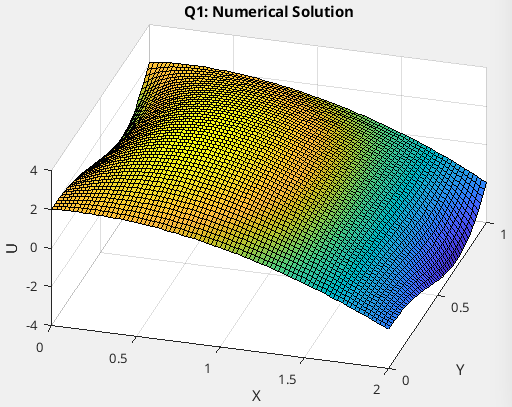
\includegraphics[width=.6\textwidth]{q1_num_sol2.png}
        \caption{Numerical Solution to (1) with $N=81, M=51$}
    \end{figure}

    \item See figure 2
    \begin{figure}[ht]
        \centering
        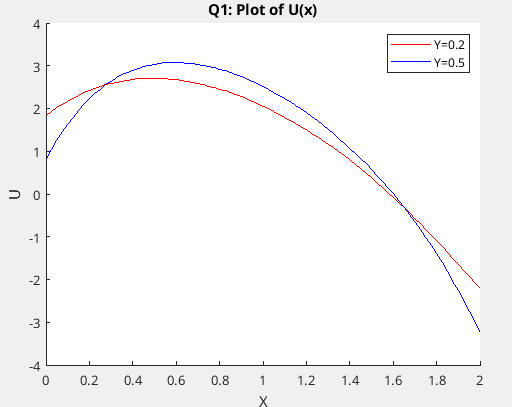
\includegraphics[width=.6\textwidth]{q1_num_sol_yconst2.png}
        \caption{Numerical Solution to (1) at $Y=0.2, 0.5$}
    \end{figure}

\end{enumerate}


\section*{Question 2: IBVP for 1D Heat Equation}

\begin{enumerate}[label=\alph*)]

    \item Determine the analytical solution for (2)
    \begin{align}
        \begin{cases}
            U_t = U_{xx}\quad \quad x \in [-1, 1],
            \quad t \ge 0\\
            U(x,0) = (3+x) + 5(1 - x^2)^2\\
            U(-1,t) = 2, \quad U(1, t) = 4
        \end{cases} 
    \end{align}
    \[
        g(x) =  3 + x + 5 - 10x^2 + 5x^4
    \]
    \begin{proof}
        To begin we look at the general solution for the Heat Equation with
        Homogeneous BC.
        \begin{align*}
            &\eta = U - 3 - x \\
            &\begin{cases}
                \eta_t = \eta_{xx} \quad \quad x \in [-1, 1],
                \quad t \ge 0\\
                \eta(x,0) = 5(1-x^2)^2\\
                \eta(-1,t) = 0, \quad \eta(1, t) = 0
            \end{cases}
        \end{align*}
        This system can be solved with the general form. 
        \begin{align*}
            \eta = \sum_n c_n\sin\left(\frac{n\pi}{2}(x+1)\right)
            e^{-\frac{n^2\pi^2}{4}t}\\
            \sum_n c_n\sin\left(\frac{n\pi}{2}(x+1)\right) = 5(1-x^2)^2\\
            c_n = \frac{2}{2}\int_{-1}^1 5(1-x^2)^2 
            \sin\left(\frac{n\pi}{2}(x+1)\right)dx \\
            c_n = 5\int_{-1}^1 (1 - 2x^2 + x^4)
            \sin\left(\frac{n\pi}{2}(x+1)\right)dx \\
        \end{align*}
        We will solve this term by term. 
        \begin{align*}
            \int_{-1}^1\sin\left(\frac{n\pi}{2}(x+1)\right)dx &= -\frac{2}{n\pi}
            \cos\left(\frac{n\pi}{2}(x+1)\right)\\
        \end{align*}
        \begin{align*}
            \int_{-1}^1x^2\sin\left(\frac{n\pi}{2}(x+1)\right)dx &= -\frac{2x^2}{n\pi}
            \cos\left(\frac{n\pi}{2}(x+1)\right) + \frac{4}{n\pi}\int_{-1}^1x\cos\left(
            \frac{n\pi}{2}(x+1)\right)dx\\
            &= -\frac{2x^2}{n\pi} \cos\left(\frac{n\pi}{2}(x+1)\right) + 
            \frac{8x}{n^2\pi^2}\sin\left(\frac{n\pi}{2}(x+1)\right) -
            \frac{8}{n^2\pi^2}\int_{-1}^1\sin\left(\frac{n\pi}{2}(x+1)\right)dx\\
            &= -\frac{2x^2}{n\pi} \cos\left(\frac{n\pi}{2}(x+1)\right) + 
            \frac{8x}{n^2\pi^2}\sin\left(\frac{n\pi}{2}(x+1)\right)
            +\frac{16}{n^3\pi^3}
            \cos\left(\frac{n\pi}{2}(x+1)\right)\\
        \end{align*}
        \begin{align*}
            \int_{-1}^1x^4\sin\left(\frac{n\pi}{2}(x+1)\right)dx &= -\frac{2x^4}{n\pi}
            \cos\left(\frac{n\pi}{2}(x+1)\right) + \frac{8}{n\pi}\int_{-1}^1x^3\cos\left(
            \frac{n\pi}{2}(x+1)\right)dx\\
            &= -\frac{2x^4}{n\pi}
            \cos\left(\frac{n\pi}{2}(x+1)\right) + \frac{16}{n^2\pi^2}x^3\sin\left(
            \frac{n\pi}{2}(x+1)\right) - \frac{48}{n^3\pi^3}\int_{-1}^1x^2\sin\left(
            \frac{n\pi}{2}(x+1)\right)dx\\
            &= -\frac{2x^4}{n\pi}
            \cos\left(\frac{n\pi}{2}(x+1)\right) + \frac{16}{n^2\pi^2}x^3\sin\left(
            \frac{n\pi}{2}(x+1)\right) \\&- \frac{48}{n^2\pi^2}\left(-\frac{2x^2}{n\pi}
            \cos\left(\frac{n\pi}{2}(x+1)\right) + 
            \frac{8x}{n^2\pi^2}\sin\left(\frac{n\pi}{2}(x+1)\right)
            +\frac{16}{n^3\pi^3}
            \cos\left(\frac{n\pi}{2}(x+1)\right)\right)\\
            &=-\frac{2x^4}{n\pi}
            \cos\left(\frac{n\pi}{2}(x+1)\right) + \frac{16}{n^2\pi^2}x^3\sin\left(
            \frac{n\pi}{2}(x+1)\right) \\
             &+\frac{96x^2}{n^3\pi^3}
            \cos\left(\frac{n\pi}{2}(x+1)\right) - 
            \frac{384x}{n^4\pi^4}\sin\left(\frac{n\pi}{2}(x+1)\right)
            +\frac{768}{n^5\pi^5}
            \cos\left(\frac{n\pi}{2}(x+1)\right)
        \end{align*}
        Obviously, terms attached to $\sin(\theta)$ will evaluate to zero, and
        terms with $\cos(\theta)$ which are multiplied by $x^k$ will be
        proportional to $\left((-1)^n -1\right)$. We have then,
        \begin{align*}
            c_n &= 5\int_{-1}^1 (1 - 2x^2 + x^4)
            \sin\left(\frac{n\pi}{2}(x+1)\right)dx \\
                &= 5\left((-1)^n -1\right)\left(-\frac{2}{n\pi} -
                2\left(-\frac{2}{n\pi} + \frac{16}{n^3\pi^3}\right)
                -\frac{2}{n\pi} +\frac{96}{n^3\pi^3}
                -\frac{768}{n^5\pi^5}\right)\\
                &= 5\left((-1)^n -1\right)\left(\frac{64}{n^3\pi^3}
                -\frac{768}{n^5\pi^5}\right)
        \end{align*}
        Thus we have found the solution to our PDE. 
        \begin{align*}
            U(x,t) = 3 + x + \sum_n 5\left((-1)^n -1\right)\left(\frac{64}{n^3\pi^3}
                -\frac{768}{n^5\pi^5}\right)\sin\left(\frac{n\pi}{2}(x+1)\right)
                e^{-\frac{n^2\pi^2}{4}t}
        \end{align*}

    \end{proof}
    \item See figure 3
    \begin{figure}[ht]
        \centering
        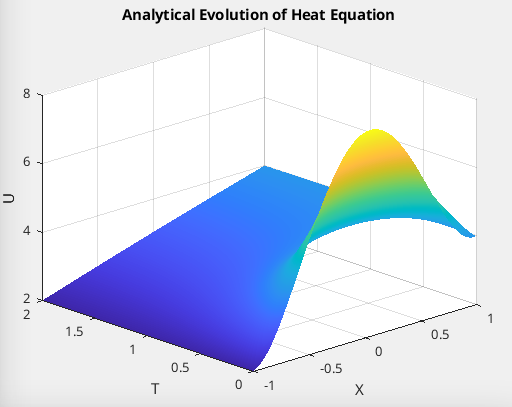
\includegraphics[width=.5\textwidth]{q2_anal_sol.png}
        \caption{Analytical Solution to (2)}
    \end{figure}

    \item See figure 4
    \begin{figure}[ht]
        \centering
        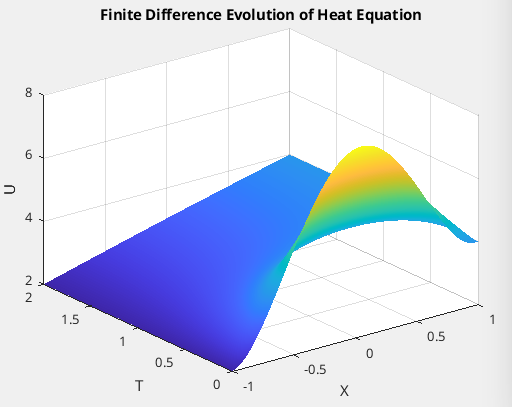
\includegraphics[width=.5\textwidth]{q2_fd_sol.png}
        \caption{Finite Solution to (2)}
    \end{figure}

    \item See figure 5
    \begin{figure}[ht]
        \centering
        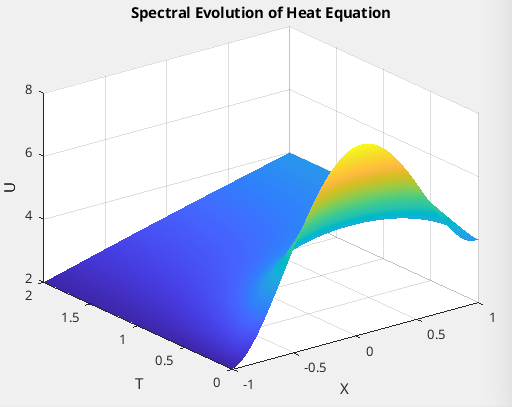
\includegraphics[width=.5\textwidth]{q2_gcl_sol.png}
        \caption{Spectral Solution to (2)}
    \end{figure}

    \item See figure 6. From the figure shown. One can deduce that initially the
    spectral method converges much more quickly. However whether due to a bug in
    my code (or seemingly every student's code) the error does not decrease
    nicely with N. In fact for larger N the error seems to rise. According to
    other students, a similar phenomenon is shown except with different orders
    of accuracy. In my figure, it seems that the Finite Diffence method
    converges with order 2, while the spectral method doesn't seem to follow any
    convergence scaling order. 
    \begin{figure}[ht]
        \centering
        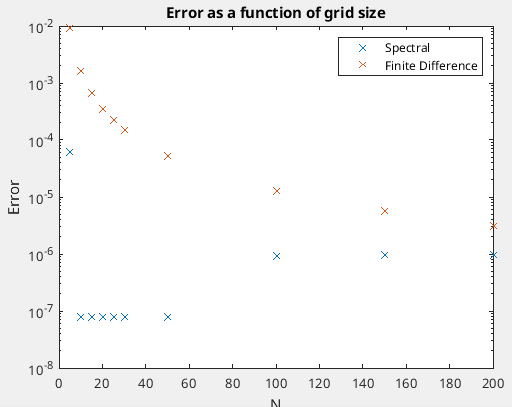
\includegraphics[width=.5\textwidth]{q2_error.png}
        \caption{Numerical Error for the FD2 and Spectral methods}
    \end{figure}

\end{enumerate}

\section*{Question 3: Extra Credit}

    \begin{align}
        \begin{cases}
            U_t +UU_{x} + U_{xx} + U_{xxxx}=0 \quad \quad x \in [-25, 25],
            \quad t \ge 0\\
            U(x,0) = \sin(x)e^{-(x-10)^2/2}\\
            U(-25,t) = U(25,t)
        \end{cases} 
    \end{align}


\begin{enumerate}[label=\alph*)]

    \item See fortran code

    \item See figure 6.
    \begin{figure}[ht]
        \centering
        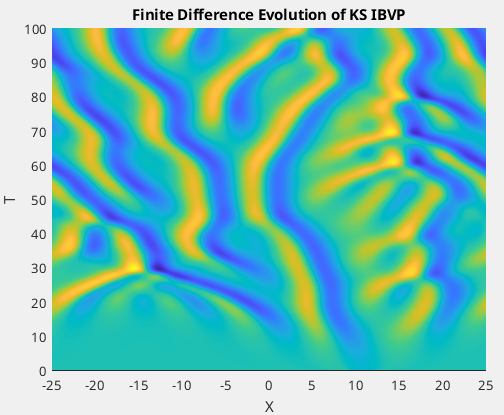
\includegraphics[width=.5\textwidth]{q3_colormap.png}
        \caption{2D Colormap of Numerical Solution to (3)}
    \end{figure}

    \item See figure 7
    \begin{figure}[ht]
        \centering
        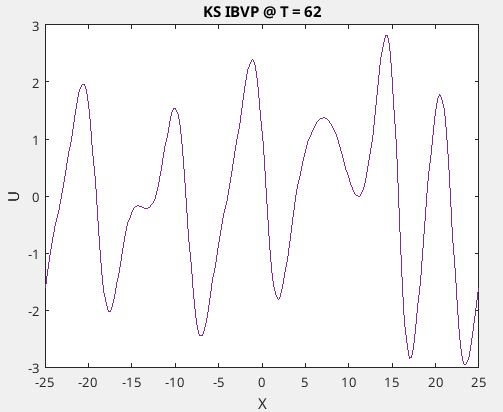
\includegraphics[width=.5\textwidth]{q3t62.png}
        \caption{Cross Section of Numerical Solution to (3) at T = 62}
    \end{figure}

\end{enumerate}

\end{document}
